\documentclass[tikz,border=10pt]{standalone}
\usepackage{amsmath}
\begin{document}
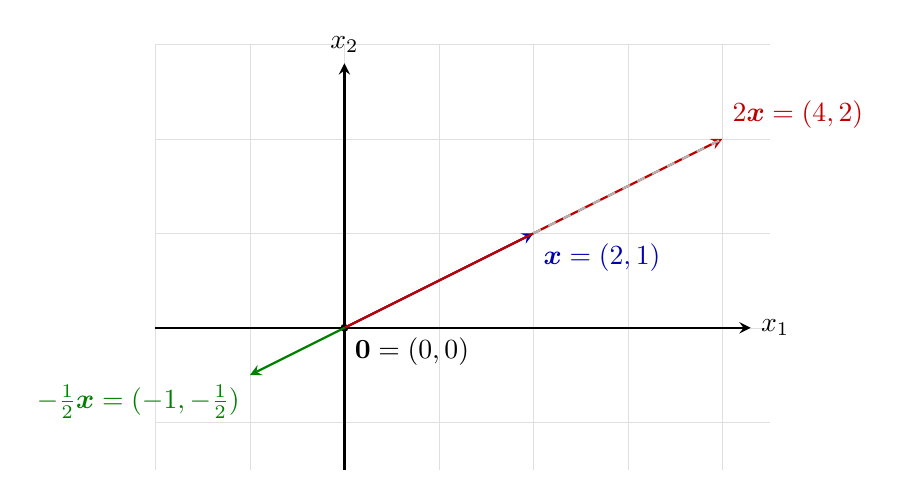
\begin{tikzpicture}[scale=1.2, >=stealth, line width=0.8pt]
  % Cuadrícula
  \draw[step=1, gray!25, very thin] (-2.0,-1.5) grid (4.5,3.0);

  % Ejes alineados con la cuadrícula
  \draw[->] (0,-1.5) -- (0,2.8) node[above] {$x_2$};
  \draw[->] (-2.0,0) -- (4.3,0) node[right] {$x_1$};

  % Origen
  \fill (0,0) circle (1.2pt) node[below right] {$\boldsymbol{0}=(0,0)$};

  % Vector original x = (2,1)
  \draw[->, thick, blue!70!black] (0,0) -- (2,1)
    node[below right] {$\boldsymbol{x}=(2,1)$};

  % 2x = (4,2)
  \draw[->, thick, red!75!black] (0,0) -- (4,2)
    node[above right] {$2\boldsymbol{x}=(4,2)$};

  % -1/2 x = (-1,-1/2)
  \draw[->, thick, green!50!black] (0,0) -- (-1,-0.5)
    node[below left] {$-\tfrac12\boldsymbol{x}=(-1,-\tfrac12)$};

  % Proyección visual
  \draw[dashed, gray!60] (2,1) -- (4,2);
\end{tikzpicture}
\end{document}
